\section{Proof of the Upper Bound}
\label{app:proof1}
In this section, we prove the upper bound of $I(H; X)$ in \multiheadname{} in Equation \ref{equ:multi_drop}.{}

\begin{figure}[H]
    \centering
    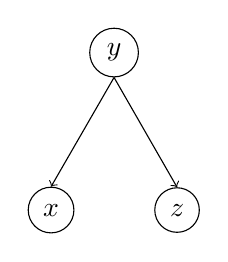
\begin{tikzpicture}[
roundnode/.style={circle,draw},
]
%Nodes
\node[roundnode]   at (0,2)   (y)                              {$y$};
\node[roundnode] at (-0.8,0)     (x)     {$x$};
\node[roundnode]   at (0.8,0)  (z)     {$z$};
%Lines
\draw[->] (y.south) -- (x.north);
\draw[->] (y.south) -- (z.north);
\end{tikzpicture}

    \caption{The graphical model of random variables $X$, $Y$ and $Z$.}
    \label{fig:graphical}
\end{figure}

\begin{lemma}
    \label{lemma:1}
    Given random variables $X$, $Y$ and $Z$. Their relationships are described in the graphical model illustrated in Figure \ref{fig:graphical}. We have
\begin{equation}
    I(X; Y | Z) \leq I(X; Y)
\end{equation}
\end{lemma}
\begin{proof}

\begin{equation}
    \begin{aligned}
I(X; &Y | Z) - I(X; Y) \\
&= \int p(x, y, z) \log \frac{p(z)p(x, y, z)}{p(x, z)p(y, z)} \mathrm{d}x \mathrm{d}z \mathrm{d}y \\ &- \int p(x, y) \log \frac{p(x, y)}{p(x)p(y)} \mathrm{d}x \mathrm{d}y\\
&=\int p(x, y, z) \log \frac{p(z)p(x, y, z)}{p(x, z)p(y, z)} \mathrm{d}x \mathrm{d}z \mathrm{d}y \\ &- \int p(x, y, z) \log \frac{p(x, y)}{p(x)p(y)} \mathrm{d}x \mathrm{d}y \mathrm{d}z\\
&=\int p(x, y, z) \log \frac{p(z)p(x,y,z)p(x)p(y)}{p(x,z)p(y,z)p(x,y)}\mathrm{d}x \mathrm{d}z \mathrm{d}y\\
&=\int p(x, y, z) \log \frac{p(z)p(x,z|y)p(y)p(x)p(y)}{p(x,z)p(y,z)p(x,y)}\mathrm{d}x \mathrm{d}z \mathrm{d}y\\
&=\int p(x, y, z) \log \frac{p(z)p(x|y)p(z|y)p(y)p(x)p(y)}{p(x,z)p(y,z)p(x,y)}\mathrm{d}x \mathrm{d}z \mathrm{d}y\\
&=\int p(x, y, z) \log \frac{p(x)p(z)}{p(x,z)}\mathrm{d}x \mathrm{d}z \mathrm{d}y\\
&=\int p(x, z) \log \frac{p(x)p(z)}{p(x,z)}\mathrm{d}x \mathrm{d}z\\
&=-I(X; Z) \leq 0
    \end{aligned}
\end{equation}
\\which finishes the proof.

\end{proof}
\begin{corollary}
\label{cor:ib}
    Given the same graphical model \ref{fig:graphical}, we have
    \begin{equation}
        I(X, Z; Y) \leq I(X; Y) + I(Z; Y)    
    \end{equation}

\end{corollary}
\begin{proof}
Using the chain rule of mutual information, we obtain
\begin{equation}
    I(X,Z;Y) = I(X;Y|Z) + I(Z; Y)
\end{equation}
According to Lemma~\ref{lemma:1}, we have $I(X; Y|Z) \leq I(X; Y)$, which finishes the proof.

\end{proof}

\begin{theorem}
    For random variables in Equation~\ref{equ:multi_drop}, we have
    \begin{equation}
        I(H;X) \leq \sum_{k=1}^K I(\boldsymbol{h}^k; X)
    \end{equation}
\end{theorem}
\begin{figure}[H]
    \centering
        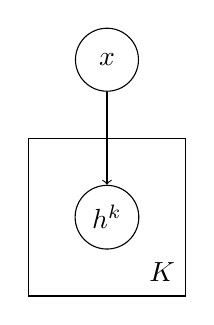
\begin{tikzpicture}[
roundnode/.style={circle,draw, minimum size=0.8cm},
]
%Nodes
\node[roundnode]   at (0,2)   (x)                              {$x$};
\node[roundnode] at (0, 0)     (hk)     {$\boldsymbol{h}^k$};
\node[draw, minimum size=2cm] at (0,0) (r) {};
\node[] at (0.7,-0.7) (t) {$K$};

%Lines
\draw[->] (x.south) -- (hk.north);
\end{tikzpicture}
    \caption{The graphical model of random variables $\boldsymbol{h}^k$ and $X$}
    \label{fig:graphical2}
\end{figure}

\begin{proof}
    According to the definitions of $X$ and $H$, which are described in Section \ref{sec:approach}, we can draw a graphical model of them in Figure~\ref{fig:graphical2}. Define a new random variable $\boldsymbol{h}^{k_1:k_2} = [\boldsymbol{h}^{k_1}, \boldsymbol{h}^{k_1+1}, \cdots, \boldsymbol{h}^{k_2-1}, \boldsymbol{h}^{k_2}]$, which is a concatenation from $\boldsymbol{h}^{k_1}$ to $\boldsymbol{h}^{k_2}$. According to Corollary~\ref{cor:ib} we have
    \begin{equation}
    \begin{aligned}
        I(H; X) &\leq I(\boldsymbol{h}^1, X) + I(\boldsymbol{h}^{2:K}, X)\\
        &\leq I(\boldsymbol{h}^1, X) + I(\boldsymbol{h}^2, X) + I(\boldsymbol{h}^{3:K}, X)\\
        &\leq I(\boldsymbol{h}^1, X) + I(\boldsymbol{h}^2, X) + I(\boldsymbol{h}^3, X) + \cdots \\
        &\leq \sum_{k=1}^K I(\boldsymbol{h}^k; X)
    \end{aligned}
    \end{equation}
\end{proof}

\begin{theorem} (proposition 1)
    \begin{equation}
            \begin{aligned}
        I(H; X)
        \leq \sum_{k=1}^K \sum_{i=1}^N
        I(\boldsymbol{h}^k_i; X_i)
        = \sum_{k=1}^K\sum_{i=1}^N \mathbb{H}[X_i] (1 - p^k_{\theta, i})
    \end{aligned}
    \end{equation}
\end{theorem}

\begin{proof}
Given \textbf{Theorem 2}. It suffices to prove
\begin{equation}
    I(\boldsymbol{h}^k; X) \leq \sum_{i=1}^N I(\boldsymbol{h}^k_i; X_i) = \sum_{i=1}^N \mathbb{H}[X_i] (1 - p^k_{\theta, i}),\quad \forall 1\leq k \leq K
\end{equation}
And this is exactly the conclusion in \cite{kim2021drop} if we consider $\boldsymbol{h}^k$ and $X$ as $X$ and $Z$ respectively in their paper.
\end{proof}

\section{Connectome-Based Predictive Modeling}
\label{sec:app_cpm}

\citet{shen2017using,finn2015functional} have shown tremendous promise in recent years in detecting imaging biomarkers by CPM (connectome-based predictive modeling) \citep{rosenberg2015predicting, dubois2018resting, rosenberg2020functional, rosenberg2016neuromarker}. Such a model, based chiefly on functional MRI data, can measure the significance of the input edge weights, which is revealed by a correlation coefficient that reflects the correlation between the edge weights and the neurological outcomes. One could expect a large correlation coefficient to indicate the high quality of edge weights. We utilize the CPM as an evaluation model to evaluate the quality of our learned hyperedges.
%The Connectome-based Predictive Modeling (CPM) pipeline is a methodological framework designed to predict neurological outcomes, such as cognitive scores, by analyzing brain connectivity.
Here is a pipeline overview of the CPM process:

\begin{enumerate}[topsep=0pt,itemsep=-1ex,partopsep=1ex,parsep=1ex]
    \item \textbf{Connectivity Calculation}: For each subject, compute the Pearson correlation coefficients for each possible pair of brain regions. This is based on the fMRI series of those regions.
    \item \textbf{Edge Significance}: Calculate the correlation between each brain connectivity edge and the outcome of interest (e.g., cognition scores) across all subjects. The correlation of an edge indicates its significance.
    \item \textbf{Edge Selection}: Identify significant connectivity edges. These are the edges where the correlation values are greater than a predetermined significance threshold.
    \item \textbf{Weight Summation}: For each subject, sum the weights of the significant edges identified in the previous step to derive a single summary score (scalar).
    \item \textbf{Model Fitting}: Fit a linear model that predicts the neurological outcomes based on the summed weights, where each subject is a sample.
    \item \textbf{Model Evaluation}: Across all subjects, calculate the correlation of predicted values and the neurological outcomes. Note that this correlation coefficient is equivalent to the one between the summed weights and the outcomes, and is exactly the metric $r$ we use to evaluate our hyperedges in Equation \ref{equ:metric}.
\end{enumerate}
Since positive edges and negative edges will cancel out with each other when being summed, we adopt the combining strategy in \cite{boyle2023connectome}.

\paragraph{CPM Measures the Quality of Edge Weights}
According to step 6, the evaluation of the predictive model could be measured by the correlation between predicted and ground-truth outcomes \cite{shen2017using}. Since CPM is a linear model that predicts the outcome based on the sum of significant edge weights, the correlation is equal to the correlation between the sum and ground-truth outcomes (which is exactly the $r$ in Equation \ref{equ:metric}). Hence, one can expect a larger correlation if the edge weights are more correlated (and thus are more predictive).

\paragraph{Significance of Edges in CPM}
In step 2, CPM obtains a correlation coefficient $r^k$ for each edge weight $w^k$ and the cognition score $Y$ across all subjects. Consider a classical hypothesis test $H_0: r^k = 0, H_1: r^k \neq 0$. Assume $w^k$ and $Y$ are drawn from independent normal distribution (corresponds to $H_0$), the probability density function of correlation coefficient $r^k$ is
$$
f(r^k)=\frac{\left(1-{r^k}^2\right)^{n / 2-2}}{\mathrm{~B}\left(\frac{1}{2}, \frac{n}{2}-1\right)},
$$
where $n$ is the number of samples and $B$ is the beta function. Based on the distribution, we obtain a $P$-value for the $k$-th edge, which is used to measure the significance of the edge.

\section{Computational Complexity}
\label{app:complexity}
Suppose we have $N$ regions as $N$ nodes and $K$ hyperedges. For the \textsc{Constructor}, the unignorable computation is from the mask operation. The computational complexity of this step for each hyperedge is $O(Nd)$ since it does a pairwise multiplication operation of a matrix of size $N \times d$. Given that there are $K$ hyperedges, the total complexity is $O(NKd)$. For the \textsc{Weighter}, the computation is from the dim reduction operation and the linear head. The dim reduction operation is an MLP. In this work, the hidden dimensions are a fraction of the original feature dimension. Therefore, the complexity of the dim-reduction MLP is $O(d^2)$. The linear head only contributes $O(d)$, which is neglectable. 
As a result, the computational complexity of the whole model is $O(NKd + d^2) = O(N^2K)$ since the feature dimension is equal to the number of regions. This complexity is just at the same scale as that of MLPs even though we are addressing a more challenging task: identifying high-order relationships in an exponential space.

\section{Dataset details}
\label{app:dataset}
\subsection{Preprocessing of ABCD Dataset}
% The functional MRI (fMRI) data is collected from children when they were resting capturing intrinsic brain activity (Rest), when they were performing the emotional n-back task (EN-back), the Stop Signal task (SST), and the Monetary Incentive Delay (MID) task.
We use the preprocessed ABIDE dataset from the official website. We preprocessed the restricted ABCD dataset ourselves. Below is the preprocessing procedure of the ABCD dataset.

\paragraph{raw data to voxel-level fMRI time series}
The fMRI data is processed using BioImage Suite \citep{joshi2011unified}. First, we performed motion correction and slice-time correction using SPM5; and via BioImage Suite, the data were registered to a standardized $3mm \times 3mm \times 3mm$ common space, where we generated masks representing white matter, gray matter, and cerebrospinal fluid (CSF) and computed the mean time courses for both white matter and CSF. We orthogonalized each gray matter time course with respect to the mean time courses of both white matter and CSF, and we orthogonalized each gray matter time course to the six motion-related signals via SPM5. We then applied a bandpass Butterworth filter with a frequency range of $0.02$Hz to $0.1$Hz to the orthogonalized time courses. We used a Gaussian kernel with a full-width at half-maximum (FWHM) of $6$mm to enhance spatial coherence and spatial smoothing. Lastly, we removed the linear trend from all signals in accordance with the methodology detailed in \cite{shenGroupwiseWholebrainParcellation2013}. We deleted scans with more than 0.10 mm mean frame-to-frame displacement. Additional details about the standard preprocessing procedures, such as slice time and motion correction, and registration to the MNI template can be found in \cite{greene2018task} and \cite{horien2019individual}.
\paragraph{voxel-level fMRI time series to region features}
The fMRI time series data of a human subject is represented in four dimensions (3 spatial dimensions + 1 temporal dimension), which can be imagined as a temporal sequence of 3D images. First, brain images are parceled into regions (or nodes) using the AAL3v1 atlas \citep{rolls2020automated}. Following previous works \citep{kan2022brain,li2021braingnn,thomas2022self}, each region's time series is obtained by averaging all voxels in that region. Consistent with previous connectivity-based methods \citep{li2021braingnn,kan2022brain,ktena2018metric,said2023neurograph}, for each region, we use its Pearson correlation coefficients to all regions as its features. We randomly split the data into train, validation, and test sets in a stratified fashion. The split ratio is 8:1:1.

\subsection{Dataset Statistics}
The statistics of the number of instances and the time series length are summarized in Table \ref{tab:stat}.
\begin{table*}
    \centering
     \caption{Statistics of datasets we use. ABIDE dataset only contains resting-state fMRI data. ABCD contains resting-state and task-based data. We use ABCD of $2$ timepoints. For example, \textit{Rest 1} means resting-state fMRI data from timepoint $1$.}
    \label{tab:stat}
    \resizebox{\textwidth}{!}{
    \begin{tabular}{ccccccccccccc}
    \toprule
          % Time Point&\multicolumn{4}{c}{1}&  &\multicolumn{4}{c}{2}\\
          % \cmidrule{2-5}\cmidrule{7-10}
          \multirow{2}{*}{Dataset} & \multicolumn{3}{c}{ABIDE} & & \multicolumn{8}{c}{ABCD} \\
          \cmidrule(lr){2-4} \cmidrule(lr){6-13}
           & FIQ & VIQ & PIQ & &Rest 1&  SST 1&  EN-back 1&  MID 1& Rest 2&  SST 2&  EN-back 2& MID 2\\
          \midrule
          \#(instances) & 1035  & 1035  & 1035&  & 1676 &  1673&  1678&  1678& 1949&  1053&  1044& 1062\\
          length of time series & 196 & 196 & 196& & 375 & 437 & 362 & 403 & 375 & 437 & 362 & 403 \\
          \bottomrule
    \end{tabular}
    }
\end{table*}


\section{Training Details}
\label{app:training}
Due to the data scarcity, we found training on single sub-datasets of the ABCD dataset leads to severe overfitting. To mitigate this, we train our model as well as all the baselines on all datasets together and report the results individually. Note that on the ABIDE dataset, we train our model under the three targets separately since we don't encounter such an issue on the ABIDE dataset.

\paragraph{Hardware}
We train our model on a machine with an Intel Xeon Gold 6326 CPU and RTX A5000 GPUs.

\paragraph{Software}
See Table \ref{tab:software} for the software we used and the versions.
\begin{table}[H]
    \centering
    \caption{Software versions.}
    \label{tab:software}
    \begin{tabular}{cc}
    \toprule
    software & version\\
    \midrule
    python & 3.8.13\\
       pytorch  & 1.11.0 \\
       cudatoolkit & 11.3 \\
       numpy  & 1.23.3 \\
       ai2-tango & 1.2.0\\
       nibabel & 4.0.2\\
       \bottomrule
    \end{tabular}
\end{table}

\paragraph{Hyperparameter Choices}
The hyperparameters selection is shown in Table \ref{tab:hyper}.

\begin{table}
    \centering
    \caption{Hyperparameter choices.}
    \label{tab:hyper}
    \begin{tabularx}{\columnwidth{}}{cXc}
    \toprule
         notation&  meaning& value\\
         \midrule
         $lr$&  learning rate& $1\times 10^{-3}$\\
         $K$&  number of hyperedges& $32$\\
         $\beta$& trade-off coefficients information bottleneck& $0.2$\\
         $[h_1, h_2, h_3]$&  hidden sizes of the dim reduction MLP& $[32,8,1]$\\
         $B$&  batch size& $64$\\
         \bottomrule
    \end{tabularx}
\end{table}

\section{Why is \textsc{HyBRiD} not the Best on the Rest 1 Dataset?}
\label{app:why_fail}
At present, we do not fully understand the reasons for the phenomena observed. The hypotheses outlined below are based on our preliminary observations and analyses.

\paragraph{Hypothesis 1: Sparsity in Resting-State Connectivity}
We propose that resting-state connectivity is sparser and more diffuse compared to task-based connectivity. This assertion is refined from our initial claim that the connectivity relevant to the phenotypic outcomes during the resting state is notably sparser than during the task-based state.

Upon examining traditional pairwise connections, we summarized the number of significant connections most related to the phenotypic outcome in Table~\ref{tab:num_sig_fail}. Our analysis indicates that Rest 1 exhibits the fewest phenotype-related connections, suggesting that these connections are indeed sparse. We did not evaluate high-order relationships due to the lack of ground truth data for such connections. Further investigation is required to validate this hypothesis. 

\begin{table}[H]
    \centering
    \begin{tabular}{c|cccccccc}
    \toprule
	& SST $1$ 	&EN-back $1$ 	&MID $1$ 	&Rest $1$ 	&SST $2$ 	&EN-back $2$ 	&MID $2$ 	&Rest $2$ \\
    \midrule
\# (connections) 	&$3164$ 	&$3414$ 	&$2989$ 	&$2036$ 	&$3112$ 	&$3014$ 	&$2692$ 	&$3896$\\
\bottomrule
    \end{tabular}
    \caption{The number of significant pairwise edges selected by CPM in different tasks and timepoints.}
    \label{tab:num_sig_fail}
\end{table}


\paragraph{Hypothesis 2: Comparative Quality of Data Across Timepoints}
We hypothesize that the data quality at timepoint 1 is inferior to that at timepoint 2. The performance metrics, as shown in the Table \ref{tab:train_test}, are better at timepoint 2 than at timepoint 1. Moreover, timepoint 1 exhibits more severe overfitting compared to timepoint 2. This discrepancy may be attributed to the higher relevance of the information (pertaining to the outcome) and lower noise levels at timepoint 2. This hypothesis also requires further verification through detailed investigations and experiments.
\begin{table}[H]
    \centering
    \begin{tabular}{c|cccccccc}
    \toprule
	&SST $1$ 	&EN-back $1$ 	&MID $1$ 	&Rest $1$ 	&SST $2$ 	&EN-back $2$ 	&MID $2$ 	&Rest $2$ \\
 \midrule
    train 	&$0.988$ 	&$0.984$ 	&$0.984$ 	&$0.984$ 	&$0.982$ 	&$0.977$ 	&$0.978$ 	&$0.976$ \\
test 	&$0.361$ 	&$0.348$ 	&$0.386$ 	&$0.223$ 	&$0.738$ 	&$0.714$ 	&$0.816$ 	&$0.730$\\
\bottomrule
    \end{tabular}
    \caption{Performances on training and test dataset in different tasks and timepoints.}
    \label{tab:train_test}
\end{table}

\paragraph{Conclusion}
Brain activities during resting states are not driven by external tasks, leading to more diffuse and less predictable patterns of activation. The low data quality of ABCD timepoint 1 (compared to timepoint 2) even intensifies this issue. Therefore, high-order relations might not be a good inductive bias on the Rest 1 dataset since the connections might be much more sparse and involve fewer nodes.

% Our model reaches the second-best on the Rest 1 dataset. To find out the reason, we inspect the performance on both the training, validation and test datasets. We summarize the performances of our model and the SOTA one in the table below
% \begin{table}[H]
%     \centering
%     \caption{Our model's performance compared to the SOTA one on the Rest 1 dataset.}
%     \label{tab:why_fail}
%     \begin{tabular}{cccc}
%     \toprule
%     model & train & validation & test \\
%     \midrule
%     BrainNetTF & $0.967$ & $0.484$ & $0.334$ \\
%     \hybrid{} (Ours)   & $0.984$ & $0.491$ & $0.223$ \\
%     \bottomrule
%     \end{tabular}
% \end{table}
% We find our model outperforms BrainNetTF on both training and validation datasets but fails on test datasets. Therefore, given that Rest 1 is the most noisy dataset, we argue that the imperfection is because

% 1) Our model overfits the training dataset more than BrainNetTF.


% 2) The validation score is higher, indicating the reason is the discrepancy between the training dataset and the test dataset.




\section{Evaluation on Synthetic Dataset}
\label{app:syn}
\paragraph{Dataset Synthesis}

\begin{table*}[htbp]
    \centering
    \caption{Precision, recall and F1 score on synthetic dataset under different $K$, where $K$ is the number of hyperedges. The performance of the Random method increases as $K$ increases because the Hungarian algorithm is likely to provide better matches when there are more candidates.}
    \label{tab:syn}
    \resizebox{\linewidth}{!}{
    \begin{tabular}{cccccccccccccccc}
    \toprule
         \multirow{2}{*}{Metric} & \multicolumn{3}{c}{$K=1$} & & \multicolumn{3}{c}{$K=5$} && \multicolumn{3}{c}{$K=10$} && \multicolumn{3}{c}{$K=30$} \\
         \cmidrule(lr){2-4}
         \cmidrule(lr){6-8}
         \cmidrule(lr){10-12}
         \cmidrule(lr){14-16}
        
         & P & R & F1 && P & R & F1&& P & R & F1& & P & R & F1  \\
         \midrule
         Random & $0.158$ & $0.094$ & $0.110$ && $0.182$ & $0.170$ & $0.171$ && $0.224$ & $0.218$ & $0.218$& & $\underline{0.288}$ & $0.250$ & $0.266$ \\
        $k$NN  & $0.533$ & $\mathbf{1.000}$ & $0.696$ && $0.247$  & $0.241$ & $0.243$ & &$0.144$ & $0.156$ & $0.148$ && $0.139$ & $0.128$ & $0.133$ \\
        $l_1$ hypergraph & $0.160$ & $\mathbf{1.000}$ & $0.276$  && $0.180$ & $0.016$ & $0.028$ && $0.135$ & $0.016$ & $0.028$ && $0.256$ & $0.026$ & $0.047$ \\
        $l_2$ hypergraph &  $\underline{0.987}$ & $0.825$  & $\underline{0.897}$ &&  $\underline{0.412}$ & $\underline{0.631}$ & $\underline{0.494}$ && $\underline{0.276}$ & $\underline{0.499}$ & $\underline{0.351}$ && $0.233$ & $\underline{0.470}$ & $0.310$ \\
        HGCN & $0.625$ & $\mathbf{1.000}$ & $0.769$  && $0.196$ & $0.477$ & $0.278$ && $0.188$ & $0.379$  & $0.251$ && $0.277$ & $0.364$ & $\underline{0.314}$  \\
        \shline
         \hybrid{} (Ours) & $\mathbf{1.000}$ & $\mathbf{1.000}$ & $\mathbf{1.000}$ && $\mathbf{0.595}$  & $\mathbf{0.680}$ & $\mathbf{0.631}$ && $\mathbf{0.504}$&$\mathbf{0.604}$ & $\mathbf{0.549}$ && $\mathbf{0.428}$ & $\mathbf{0.393}$ & $\mathbf{0.401}$ \\
         \bottomrule    
    \end{tabular}
    }
\end{table*}

Our synthetic dataset is constructed as follows:

1) \textit{Structure Generation}: For each hyperedge, we randomly sample the hyperedge degree $d$ from a discrete uniform distribution between $2$ and $d_{\text{max}}$. After that, we randomly sample $d$ nodes as members of this hyperedge. 

2) \textit{Feature generation}: For each hyperedge, we randomly sample a scalar value $v$ from the uniform distribution $U(0,1)$. We then randomly sample the features from $U(0, 2v)$ for each node in this hyperedge.

3) \textit{Label Generation}: For each hyperedge, we calculate the maximum of its node features as the summary of the hyperedge. We sum the summaries of all hyperedges to get a single value $Y$ as the label of the hypergraph. 

Note that consistent with our settings of real-world datasets, the structure is shared across all hypergraphs, while node features and hyperedge weights are different.

\paragraph{Metrics} We use the macro-precision, recall and F1 score to measure the correctness of the learned hyperedges with respect to the ground-truth ones. Note that when learning on the synthetic dataset, the order of hyperedge may differ from the ground truths. Therefore, the Hungarian algorithm is employed to match the learned hyperedges with the ground truth. The precision, recall and F1 score are calculated after matching.

\paragraph{Baselines}
We use the hyperedge construction methods in Section \ref{sec:experiments}, i.e. $k$NN\cite{huang2009video}, $l_1$ hypergraph\cite{wang2015visual} and $l_2$ hypergraph\cite{jin2019robust} as our baselines. 
Besides, we implement a hypergraph structure learning model. This is a hypergraph convolutional neural network (HGCN) \citep{bai2021hypergraph}, where both the parameters of layers and the hypergraph structure (the incidence matrix) are learnable.

\paragraph{Implementaton Details}
The maximum degree $d_{\text{max}}$ is set to $34$, which is the maximum degree of hyperedges of the ABCD dataset according to the analysis in Section \ref{sec:experiments}. The number of nodes is set to $164$, which is the number of regions of AAL3v1 atlas, used in the ABCD experiment. We conduct the experiments under different numbers of hyperedges (i.e. $K = 1,5,10,30$).

\paragraph{Results}
We report the results under different numbers of hyperedges. Although this is a hard task, our model consistently outperforms all the baselines significantly, with an average improvement of 28.3\% in terms of the F1 score. This demonstrates that our model can learn the hyperedges well under the MIMR objective, without the direct supervision of hyperedge ground truths. This also inspires us to use automated model evaluation techniques \cite{wang2023toward, peng2023came, peng2024energy} on real-world data in the future where labelled high-order relationships are not readily accessible. 


\section{Model Fit Performance}
We report the goodness of fit of our model and the state-of-the-art baseline in Table~\ref{tab:fit_abide}, with the Mean Square Error (MSE) as the metric.
\label{app:fit}
\begin{table}[H]
    \centering
    \begin{tabular}{c|ccc}
    \toprule
        Model & FIQ & VIQ & PIQ \\
    \midrule
%         BrainNetTF & $0.097$  &	$0.089$ & $0.055$ \\
% \hybrid{} (ours) & $0.057$ &	$0.071$ &	$0.046$ \\
        BrainNetTF & $5.917$  &	$5.429$ & $3.355$ \\
\hybrid{} (ours) & $\mathbf{3.477}$ &	$\mathbf{4.331}$ &	$\mathbf{2.806}$ \\
\bottomrule
    \end{tabular}
    \caption{Performance of the model and baselines (MSE) in fitting the target on the ABIDE dataset. }
    \label{tab:fit_abide}
\end{table}
% \todo{bolden and multiply the numbers by 61}

\begin{table}[H]
    \centering
    \begin{tabular}{c|cccccccc}
    \toprule
Model &	SST 1 &	EN-back 1 &	MID 1 &	Rest 1 &	SST 2 &	EN-back 2 &	MID 2 &	Rest 2 \\
\midrule
% BrainNetTF &	0.0189 &	0.0225 &	0.0188& 	0.0204& 	0.0101& 	0.0111& 	0.0118& 	0.0123 \\
% \hybrid{} (ours) & 	0.0169& 	0.0221& 	0.0209& 	0.0241& 	0.0099& 	0.0105& 	0.0089& 	0.0076 \\

BrainNetTF & 1.153 & 1.373 & $\mathbf{1.147}$ & $\mathbf{1.244}$ & 0.616 & 0.677 & 0.720 & 0.750\\
\hybrid{} (ours) &  $\mathbf{1.031}$& 	 $\mathbf{1.348}$&  $1.275$& 	 $1.470$& 	 $\mathbf{0.604}$& 	 $\mathbf{0.641}$&  $\mathbf{0.543}$& 	 $\mathbf{0.464}$ \\
\bottomrule
    \end{tabular}
    \caption{Performance of the model and baselines (MSE) in fitting the target on the ABCD dataset.}
    \label{tab:fit_abcd}
\end{table}
% \todo{bolden and multiply the numbers by 61}


\section{More Ablation Studies}
\label{app:ablation}

% \subsection{Parameters Sharing}
% \label{app:share}
% As previously discussed, the scarcity of fMRI data can result in serious over-fitting. In our experiments, we observed that when the model is trained on each dataset individually, the validation set loss remains stagnant, which indicates over-fitting. To address this, we examined the model's performance under various parameter-sharing strategies. Specifically, we have three learnable components: the shallow embeddings in Equation \ref{equ:shallow}, the dim reduction MLP in \ref{equ:readout} and the \textsc{LinearHead} $\mathcal{F}_l$. These components can be either shared or condition-specific. Results of different parameter-sharing strategy is shown in Table \ref{tab:abl_share}.

% \begin{table*}[]
%     \centering
%     \begin{tabular}{ccccc}
%     \toprule
%          Strategy ID & ShallowEmbeddings& DimReduction & LinearHead & Average Score  \\
%     \midrule
% 1&    \ding{51} & \ding{51} & \ding{51} & $0.337$ \\
% 2&    \ding{51} & \ding{51} &   & $0.335$ \\
% 3&   \ding{51} &   & \ding{51} & $0.508$ \\
% 4&    \ding{51} &      &  & $\underline{0.539}$ \\
% 5&      & \ding{51} & \ding{51} & $0.351$ \\
% 6&     & \ding{51} &  & $0.384$ \\
% 7&     &  & \ding{51} & $0.506$\\
% 8&     &  &  &  $\mathbf{0.558}$ \\
%     \bottomrule
%     \end{tabular}
%     \caption{The table summarizes the model's average performance under various parameter-sharing strategies. The symbol \ding{51} indicates a component being condition-specific, while an empty cell implies a component being shared across conditions.}
%     \label{tab:abl_share}
% \end{table*}
% Note that strategy 1 is equivalent to training models separately for each condition. From the table, we find that the DimReduction component plays the most significant role. Making DimReduction condition-specific enhances the average performance by $10\%-20\%$. Strategy 8 is the best. However, domain experts may expect different structures under different conditions. Therefore, we still adopt condition-specific ShallowEmbeddings (i.e. strategy 4), given that their scores are really close. We argue that the fact that strategy 4 is not better than strategy 8 is because our prediction target is fluid intelligence, which is a general measurement of cognition and thus tends to be condition-agnostic. We anticipate a potential shift in results if we switch to a more condition-specific cognition phenotype outcome.


\subsection{Choices of Number of Hyperedges $K$}
\label{app:k_choice}
As explained in Section \ref{sec:approach}, we use $K$ heads for $K$ hyperedges. We study the correlation between the $r$ value and the number of hyperedges on three datasets:
\begin{figure}[H]
    \begin{subfigure}[t]{0.48\linewidth}
            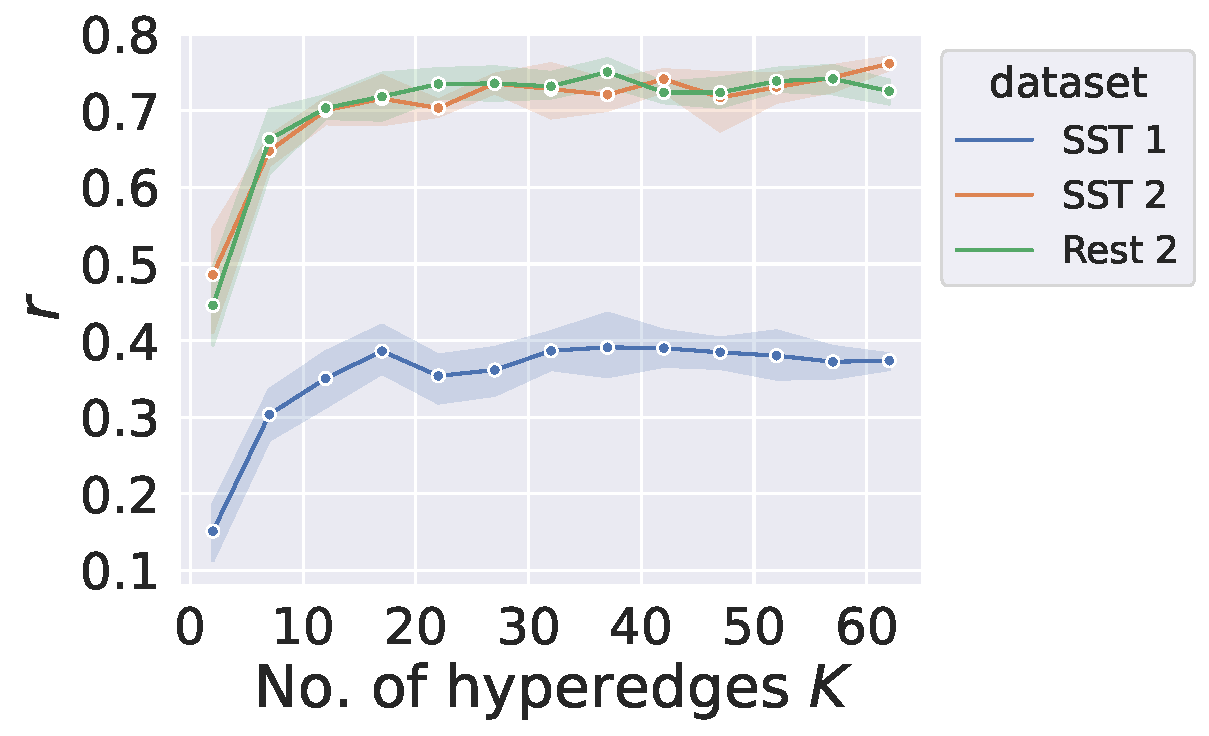
\includegraphics[width=\textwidth]{figures/ablation_mask.pdf}
    \caption{The performance with increasing the number of hyperedges through $2$, $7$, $12$, $17$, $22$, $27$, $32$, $37$, $52$, $57$, $62$ on three datasets.}
    \label{fig:abl_hyper}
    \end{subfigure}
    \hfill
    \begin{subfigure}[t]{0.48\linewidth}
    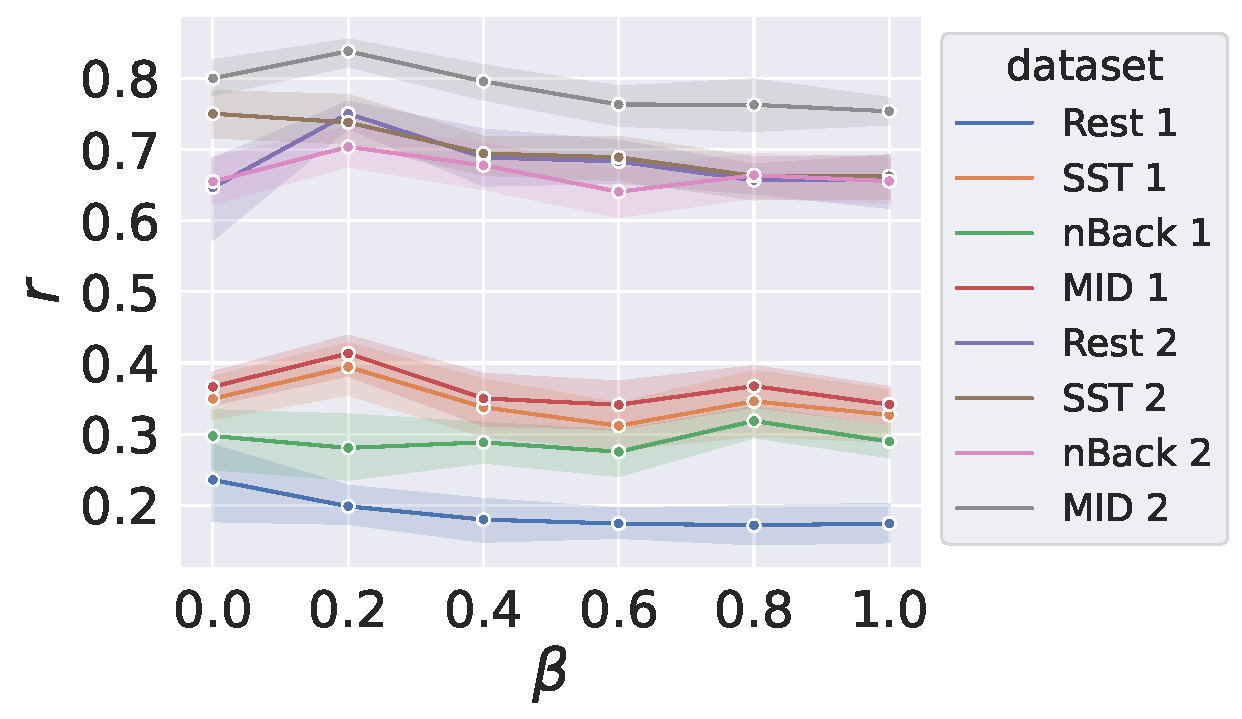
\includegraphics[width=\textwidth]{figures/ablation_beta.pdf}
    \caption{Performance with increasing $\beta$ from $0.1$ to $1.0$ with step $0.1$ on all datasets.}
    \label{fig:abl_beta}
    \end{subfigure}
    \caption{Studies on the choice of two key hyperparameters, $\beta$ and $K$, in our model.}

\end{figure}

From Figure \ref{fig:abl_hyper}, we find that the overall performance increases dramatically before $K=17$, but becomes stable and close to saturation after $K=32$. To improve the efficiency while ensuring the performance, we choose $K=32$.

\subsection{Choices of the Trade-off Coefficient $\beta$}
\label{app:beta}

In our optimization objective \ref{equ:ib2}, $\beta$ acts as a trade-off parameter, which is a non-negative scalar that determines the weight given to the second term relative to the first. To study its fluence to the performance, we plot the model performances on all datasets under different $\beta$ in Figure \ref{fig:abl_beta}. We can see performances on $3$ datasets (Rest 1, SST 2) consistently decrease when $\beta$ increases. However, on other $5$ datasets (SST 1, MID 1, Rest 2, nBack 2, MID 2), we can observe a peak at $\beta=0.2$. Accordingly, we adopt $\beta=0.2$.

% \section{Region Importance}
% To better understand each brain region's role in cognition under different conditions. We define the region importance as how many times it gets involved (participates) in a hyperedge. The more it participates, the more important it should be considered. We rank these regions by their importance in Figure \ref{fig:region_importance}. 

% \label{app:region_importance}
% \begin{figure}
% \begin{subfigure}[b]{0.48\textwidth}
%     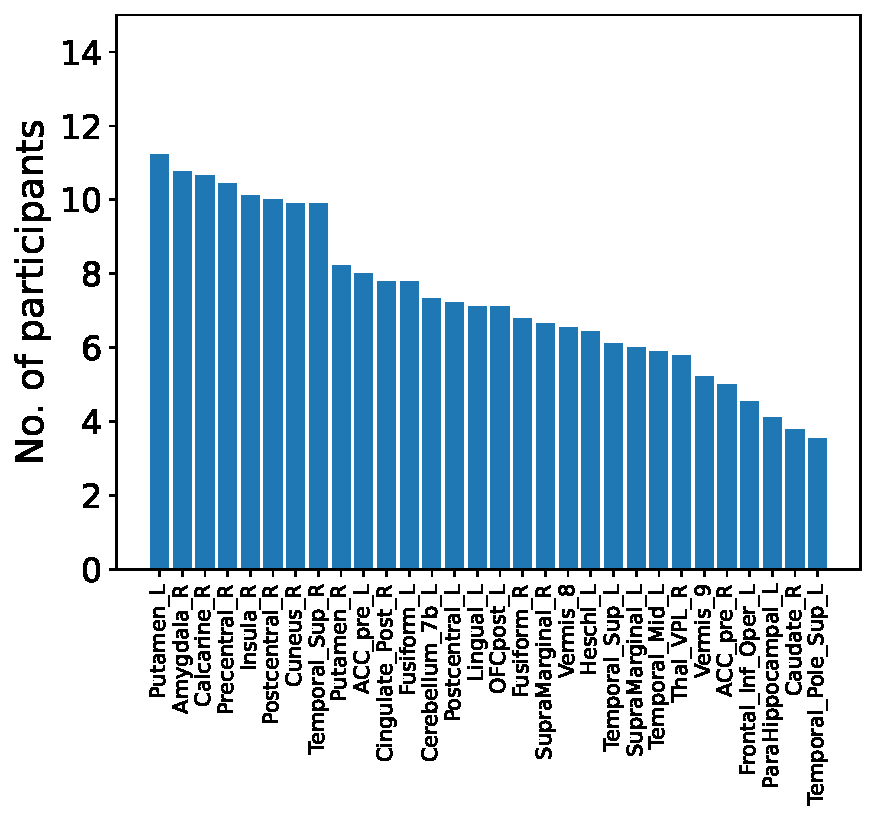
\includegraphics[width=\textwidth]{figures/most_Rest_participants.pdf}
%     \caption{Node importance ranking of Rest.}
% \end{subfigure}
% \begin{subfigure}[b]{0.48\textwidth}
%     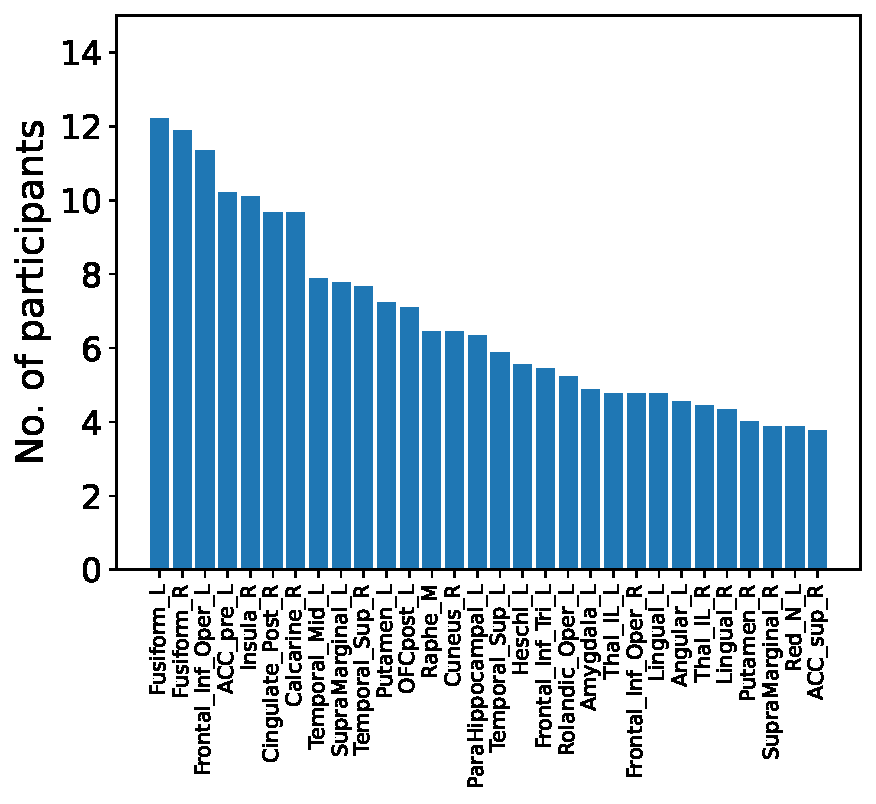
\includegraphics[width=\textwidth]{figures/most_SST_participants.pdf}
%     \caption{Node importance ranking of SST.}
% \end{subfigure}
% \begin{subfigure}[b]{0.48\textwidth}
%     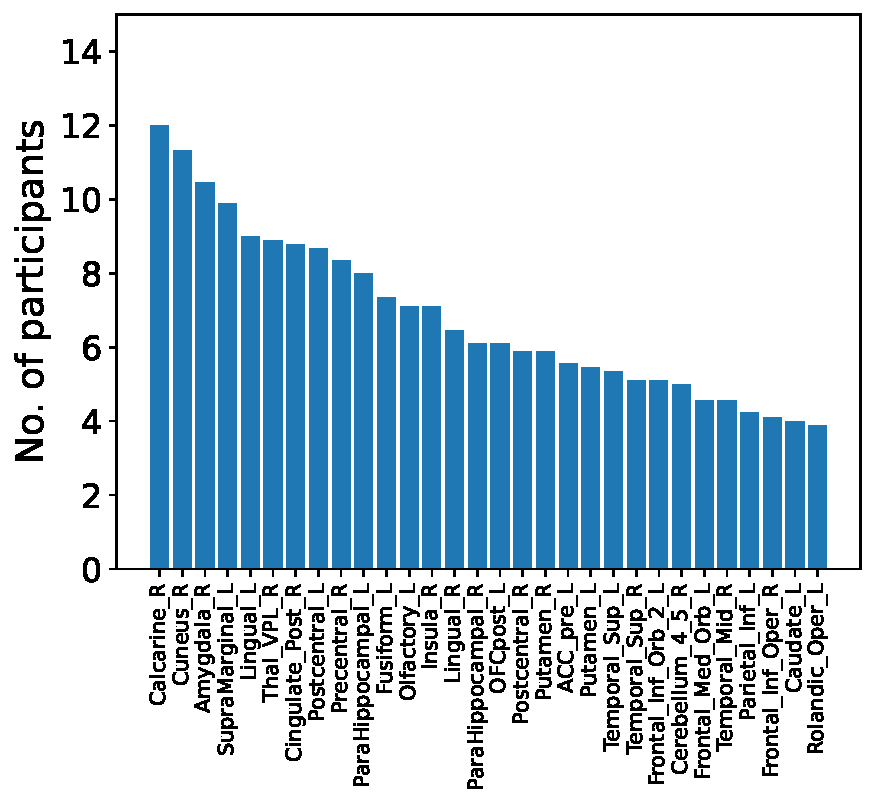
\includegraphics[width=\textwidth]{figures/most_nBack_participants.pdf}
%     \caption{Node importance ranking of EN-back.}
% \end{subfigure}\begin{subfigure}[b]{0.48\textwidth}
%     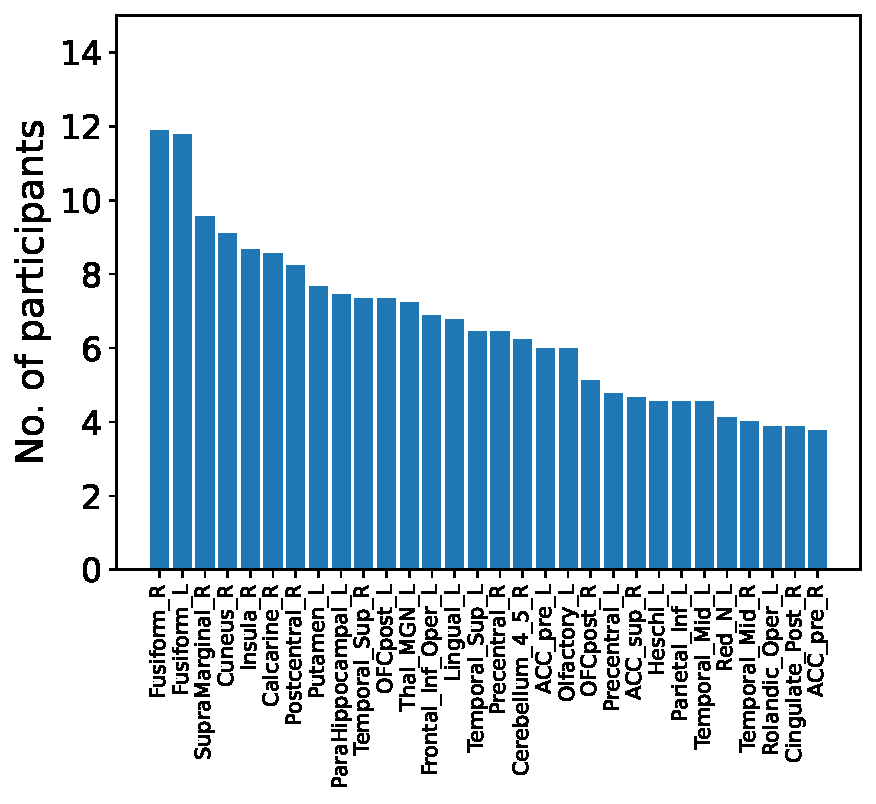
\includegraphics[width=\textwidth]{figures/most_MID_participants.pdf}
%     \caption{Node importance ranking of MID.}
% \end{subfigure}
% \caption{Node importance ranking under different conditions.}
% \label{fig:region_importance}
% \end{figure}

\section{Runtime Comparison}
\label{app:runtime}
Figure \ref{fig:runtime} summarizes the per-batch training time of all deep learning models. We find that \hybrid{} is the most efficient one, with $87\%$ faster than the second one (BrainNetTF) and at least $1255\%$ faster than the GNN-based ones.

\begin{figure}[H]
    \centering
    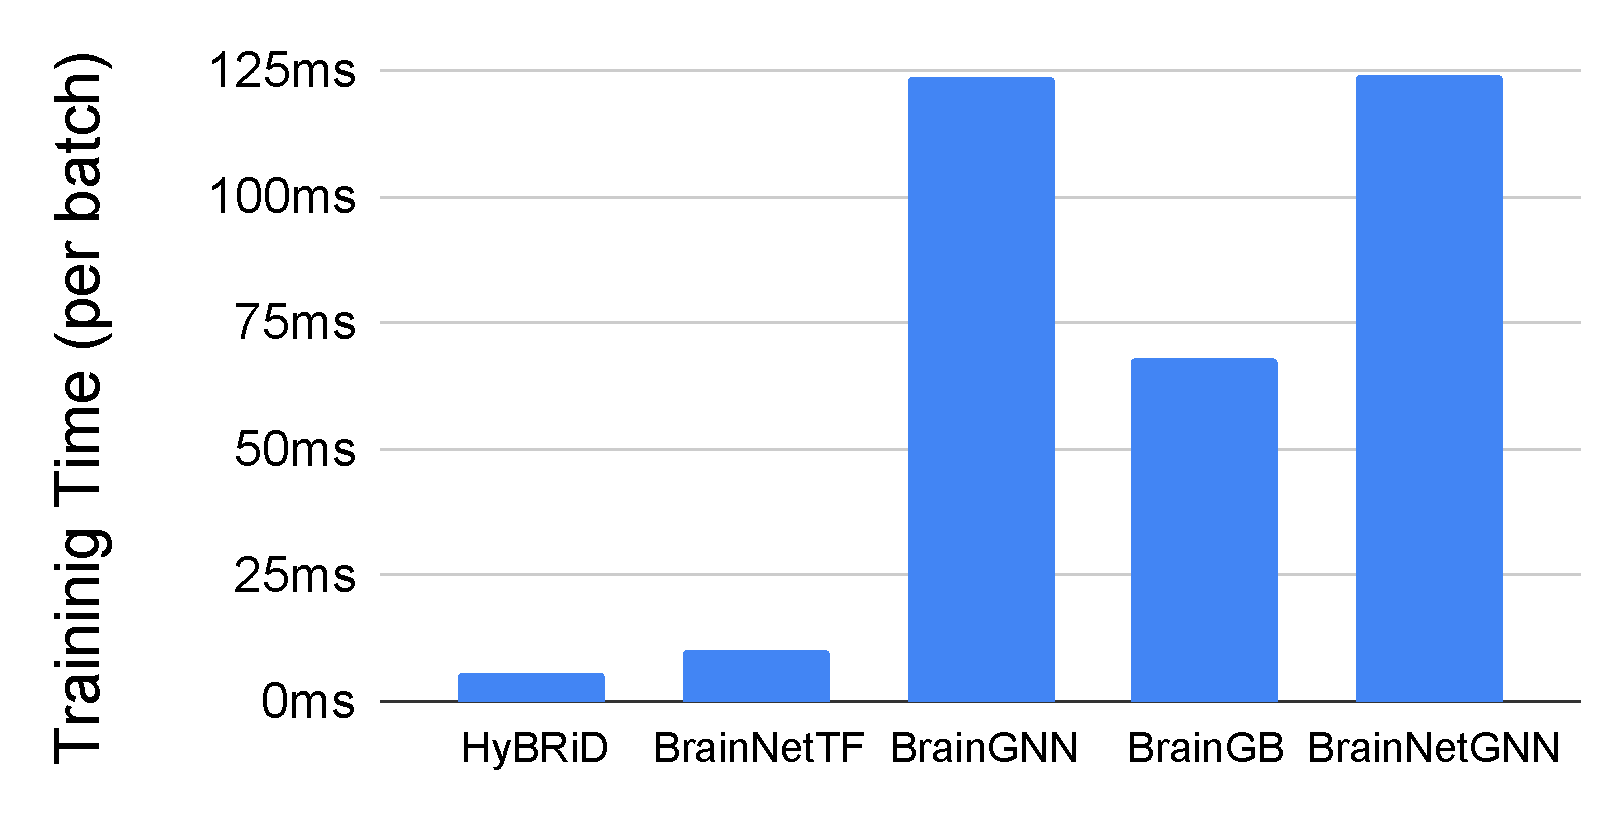
\includegraphics[width=0.5\linewidth]{figures/runtime.pdf}
    \caption{Training time per batch of all deep learning models.}
    \label{fig:runtime}
\end{figure}


\section{More Visualizations}
\label{app:viz}
\paragraph{Task-Based Brain Region Importance}
\begin{figure}
    \centering
    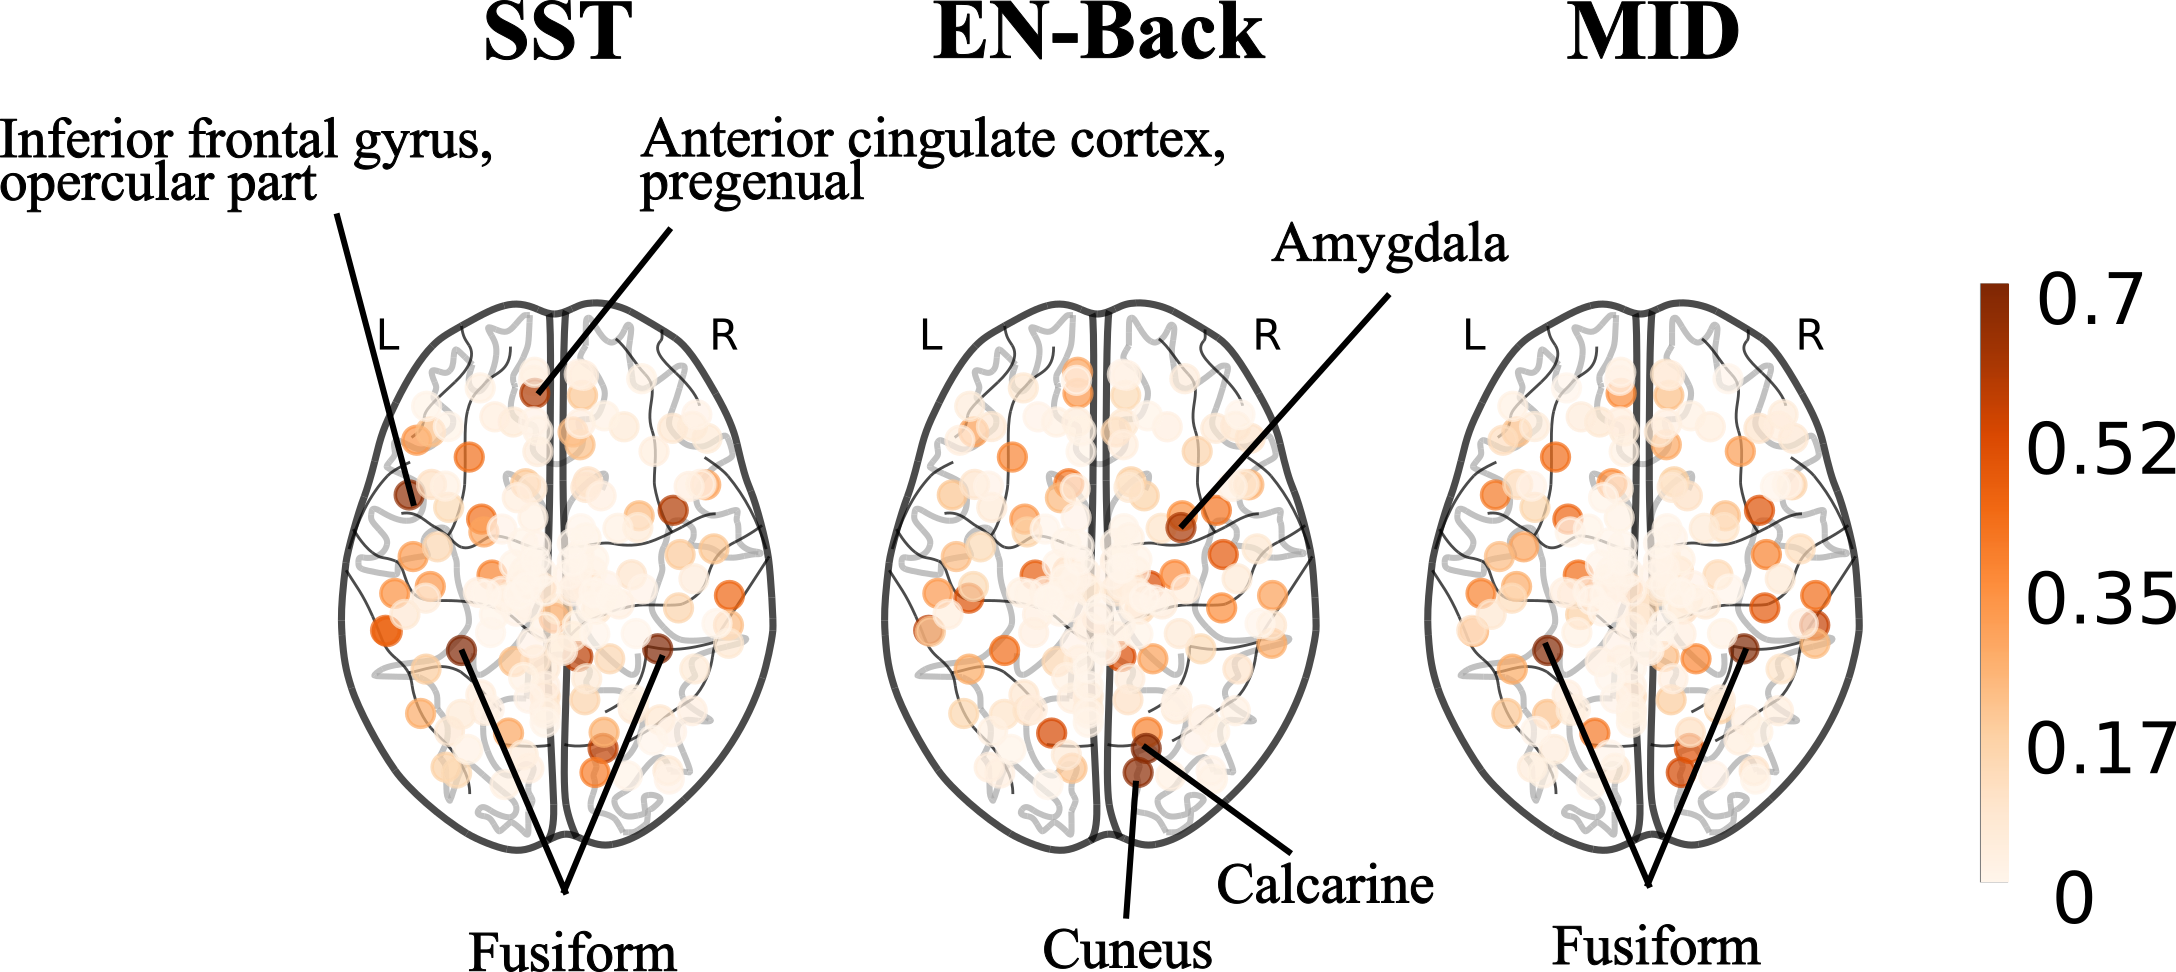
\includegraphics[width=0.49\textwidth]{figures/brainregionplot.png}
    \vskip 0.1in
    \caption{Visualization of the frequency of each region under different fMRI tasks.}
    \label{fig:brainplot}
    \vskip -0.1in
\end{figure}
To better understand the roles of each brain region in cognition under different fMRI tasks, we study the frequency at which each region appears in a hyperedge out of all identified hyperedges. The frequency, which can be considered as a measure of region importance, is visualized in Figure \ref{fig:brainplot}.
Visual regions (\textit{Fusiform}, \textit{Cuneus}, \textit{Calcarine}) are especially active due to the intensive visual demands in all three tasks.
We found that the \textit{Inferior frontal gyrus, opercular part} and the \textit{Anterior cingulate cortex, pregenual}, recognized for their participation in response inhibition \citep{pornpattananangkul2016cultural}, frequently appear in the SST task. This aligns with what the SST task was designed to test. Interestingly, of the three tasks (SST, EN-back, MID), only EN-back prominently involves the \textit{Amygdala}, a key region for emotion processing. This makes sense as EN-back is the only task related to emotion. 


\paragraph{Resting-State Brain Region Importance}
We visualize the region importance of the resting state in Figure \ref{fig:rest_region}. Different from task states, where specific brain regions are activated in response to particular tasks, brain activities during resting states, are not driven by external tasks, leading to more diffuse and less predictable patterns of activation. This makes it harder to pinpoint specific interactions or functions.
\begin{figure}[H]
    \centering
    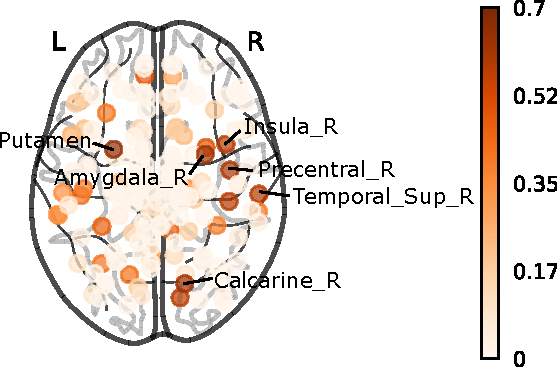
\includegraphics[width=0.4\linewidth]{figures/Rest.pdf}
    \caption{Region importance of resting state.}
    \label{fig:rest_region}
\end{figure}


% Sensory Integration: The presence of primary sensory areas (like the Calcarine, associated with vision) and association areas suggests that sensory information is being integrated with higher-order cognitive processes, perhaps as the subject views and responds to emotional images or words.
% \section{Limitations}
% \label{app:limitations}
% \hybrid{} only considers static high-order relations. Given that ABCD tasks are dynamic, including temporal changes and interactions, it will be interesting to study the evolution of these high-order relationships.


\section{Discussion of the Possible Methods to Interpret Hyperedges}
\label{app:interpret}
As mentioned in the main text, high-order relationships are much harder to interpret than pairwise ones given the exponential complexity. Here we propose a potential hierarchical strategy that tries to interpret them.

\begin{itemize}
    \item  \textbf{Adaptive Clustering Algorithm with Adjustable Granularity}: Suppose we have a clustering algorithm, where the granularity (or number of clusters) can be controlled. The clustering algorithm can cluster brain regions based on their functions (e.g. motor, visual, …) to different function modules \cite{shen2010graph}.
    \item   \textbf{Initial Analysis at Lower Granularity}: Set the granularity at a low level (i.e. small number of clusters). In this case, the high-order relationships are much easier to interpret (since the degree is low). However, some high-order relationships will connect to the same set of clusters, thus implying the interactions between the same set of function modules. For example, high-order relations $h_1$ and $h_2$ both connect to visual, motor, and emotion.
    \item \textbf{Refinement through Increased Granularity}: Find the high-order relationships that connect to the same set of function modules, and increase the granularity level, so we can tell the difference between them. For example, $h1$ may connect to the left part of the visual module, while $h_2$ connects to the right part.
\end{itemize}